% Options for packages loaded elsewhere
\PassOptionsToPackage{unicode}{hyperref}
\PassOptionsToPackage{hyphens}{url}
\PassOptionsToPackage{dvipsnames,svgnames,x11names}{xcolor}
%
\documentclass[
  letterpaper,
  DIV=11,
  numbers=noendperiod]{scrartcl}

\usepackage{amsmath,amssymb}
\usepackage{iftex}
\ifPDFTeX
  \usepackage[T1]{fontenc}
  \usepackage[utf8]{inputenc}
  \usepackage{textcomp} % provide euro and other symbols
\else % if luatex or xetex
  \usepackage{unicode-math}
  \defaultfontfeatures{Scale=MatchLowercase}
  \defaultfontfeatures[\rmfamily]{Ligatures=TeX,Scale=1}
\fi
\usepackage{lmodern}
\ifPDFTeX\else  
    % xetex/luatex font selection
\fi
% Use upquote if available, for straight quotes in verbatim environments
\IfFileExists{upquote.sty}{\usepackage{upquote}}{}
\IfFileExists{microtype.sty}{% use microtype if available
  \usepackage[]{microtype}
  \UseMicrotypeSet[protrusion]{basicmath} % disable protrusion for tt fonts
}{}
\makeatletter
\@ifundefined{KOMAClassName}{% if non-KOMA class
  \IfFileExists{parskip.sty}{%
    \usepackage{parskip}
  }{% else
    \setlength{\parindent}{0pt}
    \setlength{\parskip}{6pt plus 2pt minus 1pt}}
}{% if KOMA class
  \KOMAoptions{parskip=half}}
\makeatother
\usepackage{xcolor}
\setlength{\emergencystretch}{3em} % prevent overfull lines
\setcounter{secnumdepth}{5}
% Make \paragraph and \subparagraph free-standing
\ifx\paragraph\undefined\else
  \let\oldparagraph\paragraph
  \renewcommand{\paragraph}[1]{\oldparagraph{#1}\mbox{}}
\fi
\ifx\subparagraph\undefined\else
  \let\oldsubparagraph\subparagraph
  \renewcommand{\subparagraph}[1]{\oldsubparagraph{#1}\mbox{}}
\fi


\providecommand{\tightlist}{%
  \setlength{\itemsep}{0pt}\setlength{\parskip}{0pt}}\usepackage{longtable,booktabs,array}
\usepackage{calc} % for calculating minipage widths
% Correct order of tables after \paragraph or \subparagraph
\usepackage{etoolbox}
\makeatletter
\patchcmd\longtable{\par}{\if@noskipsec\mbox{}\fi\par}{}{}
\makeatother
% Allow footnotes in longtable head/foot
\IfFileExists{footnotehyper.sty}{\usepackage{footnotehyper}}{\usepackage{footnote}}
\makesavenoteenv{longtable}
\usepackage{graphicx}
\makeatletter
\def\maxwidth{\ifdim\Gin@nat@width>\linewidth\linewidth\else\Gin@nat@width\fi}
\def\maxheight{\ifdim\Gin@nat@height>\textheight\textheight\else\Gin@nat@height\fi}
\makeatother
% Scale images if necessary, so that they will not overflow the page
% margins by default, and it is still possible to overwrite the defaults
% using explicit options in \includegraphics[width, height, ...]{}
\setkeys{Gin}{width=\maxwidth,height=\maxheight,keepaspectratio}
% Set default figure placement to htbp
\makeatletter
\def\fps@figure{htbp}
\makeatother
\newlength{\cslhangindent}
\setlength{\cslhangindent}{1.5em}
\newlength{\csllabelwidth}
\setlength{\csllabelwidth}{3em}
\newlength{\cslentryspacingunit} % times entry-spacing
\setlength{\cslentryspacingunit}{\parskip}
\newenvironment{CSLReferences}[2] % #1 hanging-ident, #2 entry spacing
 {% don't indent paragraphs
  \setlength{\parindent}{0pt}
  % turn on hanging indent if param 1 is 1
  \ifodd #1
  \let\oldpar\par
  \def\par{\hangindent=\cslhangindent\oldpar}
  \fi
  % set entry spacing
  \setlength{\parskip}{#2\cslentryspacingunit}
 }%
 {}
\usepackage{calc}
\newcommand{\CSLBlock}[1]{#1\hfill\break}
\newcommand{\CSLLeftMargin}[1]{\parbox[t]{\csllabelwidth}{#1}}
\newcommand{\CSLRightInline}[1]{\parbox[t]{\linewidth - \csllabelwidth}{#1}\break}
\newcommand{\CSLIndent}[1]{\hspace{\cslhangindent}#1}

\usepackage{booktabs}
\usepackage{longtable}
\usepackage{array}
\usepackage{multirow}
\usepackage{wrapfig}
\usepackage{float}
\usepackage{colortbl}
\usepackage{pdflscape}
\usepackage{tabu}
\usepackage{threeparttable}
\usepackage{threeparttablex}
\usepackage[normalem]{ulem}
\usepackage{makecell}
\usepackage{xcolor}
\usepackage{caption}
\KOMAoption{captions}{tableheading}
\makeatletter
\makeatother
\makeatletter
\makeatother
\makeatletter
\@ifpackageloaded{caption}{}{\usepackage{caption}}
\AtBeginDocument{%
\ifdefined\contentsname
  \renewcommand*\contentsname{Table of contents}
\else
  \newcommand\contentsname{Table of contents}
\fi
\ifdefined\listfigurename
  \renewcommand*\listfigurename{List of Figures}
\else
  \newcommand\listfigurename{List of Figures}
\fi
\ifdefined\listtablename
  \renewcommand*\listtablename{List of Tables}
\else
  \newcommand\listtablename{List of Tables}
\fi
\ifdefined\figurename
  \renewcommand*\figurename{Figure}
\else
  \newcommand\figurename{Figure}
\fi
\ifdefined\tablename
  \renewcommand*\tablename{Table}
\else
  \newcommand\tablename{Table}
\fi
}
\@ifpackageloaded{float}{}{\usepackage{float}}
\floatstyle{ruled}
\@ifundefined{c@chapter}{\newfloat{codelisting}{h}{lop}}{\newfloat{codelisting}{h}{lop}[chapter]}
\floatname{codelisting}{Listing}
\newcommand*\listoflistings{\listof{codelisting}{List of Listings}}
\makeatother
\makeatletter
\@ifpackageloaded{caption}{}{\usepackage{caption}}
\@ifpackageloaded{subcaption}{}{\usepackage{subcaption}}
\makeatother
\makeatletter
\@ifpackageloaded{tcolorbox}{}{\usepackage[skins,breakable]{tcolorbox}}
\makeatother
\makeatletter
\@ifundefined{shadecolor}{\definecolor{shadecolor}{rgb}{.97, .97, .97}}
\makeatother
\makeatletter
\makeatother
\makeatletter
\makeatother
\ifLuaTeX
  \usepackage{selnolig}  % disable illegal ligatures
\fi
\IfFileExists{bookmark.sty}{\usepackage{bookmark}}{\usepackage{hyperref}}
\IfFileExists{xurl.sty}{\usepackage{xurl}}{} % add URL line breaks if available
\urlstyle{same} % disable monospaced font for URLs
\hypersetup{
  pdftitle={How did local health infrastructure and socio-political factors within different states and counties in the United States affect the disparities in COVID-19 outcomes, and what lessons can be learned for more targeted public health preparedness and response strategies in future pandemics?},
  pdfauthor={Adrian Ly; Sakhil Goel; Hannah Yu},
  colorlinks=true,
  linkcolor={blue},
  filecolor={Maroon},
  citecolor={Blue},
  urlcolor={Blue},
  pdfcreator={LaTeX via pandoc}}

\title{How did local health infrastructure and socio-political factors
within different states and counties in the United States affect the
disparities in COVID-19 outcomes, and what lessons can be learned for
more targeted public health preparedness and response strategies in
future pandemics?\thanks{Code and data are available at:
https://github.com/hannahyu07/US-Covid-Analysis.git}}
\author{Adrian Ly \and Sakhil Goel \and Hannah Yu}
\date{February 13, 2024}

\begin{document}
\maketitle
\begin{abstract}
First sentence. Second sentence. Third sentence. Fourth sentence.
\end{abstract}
\ifdefined\Shaded\renewenvironment{Shaded}{\begin{tcolorbox}[breakable, borderline west={3pt}{0pt}{shadecolor}, boxrule=0pt, frame hidden, enhanced, interior hidden, sharp corners]}{\end{tcolorbox}}\fi

\renewcommand*\contentsname{Table of contents}
{
\hypersetup{linkcolor=}
\setcounter{tocdepth}{3}
\tableofcontents
}
\hypertarget{introduction}{%
\section{Introduction}\label{introduction}}

\emph{This reproduction was performed after a replication on the Social
Science Reproduction platform:
}\textbf{\emph{\href{https://www.socialsciencereproduction.org/reproductions/c35e8e98-762d-4c00-a1a3-544ed0b2008d/index}{link
here}}}

Figure~\ref{fig-GHS} allows us to visualize the Global Health Security
(GHS) Index which is designed to assess a country's capabilities to
prevent, detect, and respond to significant infectious disease
outbreaks. A higher Global Health Security (GHS) Index score indicates a
stronger health system capacity for pandemic readiness. The GHS Index
assesses the readiness of countries for pandemics and other significant
biological threat emergencies, using a comprehensive framework that
includes measurements grouped into six broad categories: prevention,
detection, response, health system capacity, compliance with
international norms, and risk environment. Higher scores suggest that a
country has a more robust health system capacity, with better
capabilities to prevent, detect, respond to, and mitigate the spread of
an epidemic.

Conversely, a lower GHS Index score implies weaker health system
capacities, suggesting that the country may be less prepared to handle
pandemics and other significant biological threats. Lower scores
indicate deficiencies in one or more of the critical areas assessed by
the Index, which could potentially hinder the country's ability to
effectively manage and control the spread of infectious diseases.

\begin{figure}

{\centering 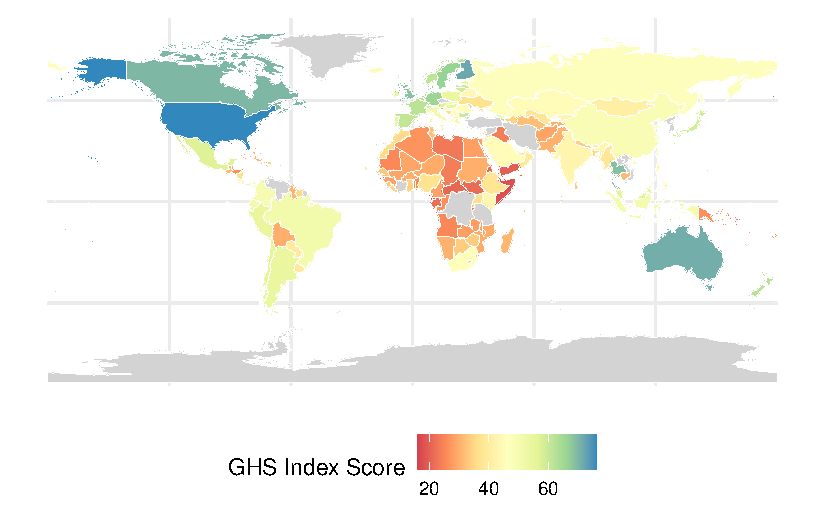
\includegraphics{paper_files/figure-pdf/fig-GHS-1.pdf}

}

\caption{\label{fig-GHS}Global Health Security Index Scores by Country}

\end{figure}

\hypertarget{sec-data}{%
\section{Data}\label{sec-data}}

\hypertarget{source}{%
\subsection{Source}\label{source}}

The datasets utilized in this paper were mainly obtained from the
\texttt{original\ paper} (Nuzzo and Ledesma 2023). The data used by the
paper was compiled from various sources such as the Arias et al. (2022),
Arias and Xu (2022), Bell and Nuzzo (2021), Systems Science and
Engineering (2023), Dong, Du, and Gardner (2020), \emph{COVID-19 Excess
Mortality Estimates 2020-2021} (2022), Ledesma et al. (2023), Health
Statistics (2022), {``Death Rate, Crude (Per 1,000 People)
(SP.DYN.CDRT.IN)''} (2022), Economic and Division (2022), and Wang et
al. (2022). Additionally, to address the original paper's lack of US
COVID statistics and political party support data, we incorporated
information from Jack and Oster (2023) and (Elflein 2023). The political
party support data we utilized from Jack and Oster (2023) was compiled
from McGovern (2009-\/-2020).

Jack and Oster (2023) discusses the long-term impacts of COVID-related
school closures. From this source, we utilized the dataset on voting
shares during the 2020 election by county. Elflein (2023) summarizes
COVID-19 death rates in the United States as of March 2023, organized by
state. Analyzing results from both datasets allows us to explore the
relationship between political affiliation and COVID-19 outcomes. Our
reproduction aims to fill these gaps and includes tables and graphs not
presented in the original paper to support our findings.

\hypertarget{methodology}{%
\subsection{Methodology}\label{methodology}}

This paper will replicate the data that was originally presented by
Nuzzo and Ledesma (2023), as previously mentioned. We then transform the
replication to our data analysis incorporating the COVID statistics and
political party support data. We seek to use our initial replication and
following own data analysis to provide a fresh part of the original
paper, enhancing the with more data. Different from the original paper
which spent a lot of time talking about how badly prepared the US was
against other countries, We also specifically diverge our focus to the
political and socioeconomic factors that impacted the US's COVID
outcome.

\texttt{R} (R Core Team 2022) was the language and environment used for
the bulk of this analysis, alongside \texttt{tidyverse} (Wickham et al.
2019), \texttt{sf} (Pebesma 2018), \texttt{readxl} (Wickham and Bryan
2023), \texttt{knitr} (Xie 2014), \texttt{janitor} (Firke 2023),
\texttt{lubridate} (Grolemund and Wickham 2011), \texttt{dplyr} (Wickham
et al. 2023), \texttt{data.table} (Barrett et al. 2024),
\texttt{RColorBrewer} (Neuwirth 2022), \texttt{ggpubr} (Kassambara
2023), \texttt{ggplot2} (Wickham 2016), \texttt{here} (Müller 2020),
\texttt{kableExtra} (Zhu 2024), \texttt{webshot} (Chang 2023a),
\texttt{webshot2} (Chang 2023b), \texttt{gt} (Iannone et al. 2024) and
\texttt{scales} (Wickham, Pedersen, and Seidel 2023).

\hypertarget{data-cleaning}{%
\subsection{Data cleaning}\label{data-cleaning}}

From all the data provided from Nuzzo and Ledesma (2023), Jack and Oster
(2023), and Elflein (2023), we mainly utilize Bell and Nuzzo (2021),
Health Statistics (2022), McGovern (2009-\/-2020), and Elflein (2023).
The data from Nuzzo and Ledesma (2023) is well-organized and require
minimal cleaning for analysis.

The data collected from McGovern (2009-\/-2020) is at the county level
as depicted on Table~\ref{tbl-sample}. However, since our analysis
focuses on people's political preferences at the state level, we create
a new data frame called ``vote\_data\_by\_state'' to aggregate voting
data by state. We utilize the ``group\_by'' function to generate new
variables at the state level, calculating the total votes, total
Republican party votes, total Democratic party votes, and the total vote
difference between the two parties by county. Additionally, We also
create variables for the average percentage of votes each party receives
and the difference by each state.

To determine the total number of votes in the Top 10 states with the
highest proportion of Republican votes, we create another new data frame
called ``sorted\_states'' from the ``vote\_data\_by\_state'' data frame.
We include a new variable ``proportion\_republican'' that calculates the
proportion of votes the Republican party receives from each state and
orders the states by the highest proportion of Republican votes.

\hypertarget{tbl-sample}{}
\begin{longtable}[]{@{}
  >{\raggedright\arraybackslash}p{(\columnwidth - 18\tabcolsep) * \real{0.0791}}
  >{\raggedleft\arraybackslash}p{(\columnwidth - 18\tabcolsep) * \real{0.0863}}
  >{\raggedright\arraybackslash}p{(\columnwidth - 18\tabcolsep) * \real{0.1079}}
  >{\raggedleft\arraybackslash}p{(\columnwidth - 18\tabcolsep) * \real{0.0719}}
  >{\raggedleft\arraybackslash}p{(\columnwidth - 18\tabcolsep) * \real{0.0719}}
  >{\raggedleft\arraybackslash}p{(\columnwidth - 18\tabcolsep) * \real{0.0863}}
  >{\raggedleft\arraybackslash}p{(\columnwidth - 18\tabcolsep) * \real{0.0791}}
  >{\raggedleft\arraybackslash}p{(\columnwidth - 18\tabcolsep) * \real{0.1079}}
  >{\raggedleft\arraybackslash}p{(\columnwidth - 18\tabcolsep) * \real{0.1079}}
  >{\raggedleft\arraybackslash}p{(\columnwidth - 18\tabcolsep) * \real{0.2014}}@{}}
\caption{\label{tbl-sample}Sample of Vote Share Data}\tabularnewline
\toprule\noalign{}
\begin{minipage}[b]{\linewidth}\raggedright
State Name
\end{minipage} & \begin{minipage}[b]{\linewidth}\raggedleft
County FIPS
\end{minipage} & \begin{minipage}[b]{\linewidth}\raggedright
County Name
\end{minipage} & \begin{minipage}[b]{\linewidth}\raggedleft
Votes GOP
\end{minipage} & \begin{minipage}[b]{\linewidth}\raggedleft
Votes DEM
\end{minipage} & \begin{minipage}[b]{\linewidth}\raggedleft
Total Votes
\end{minipage} & \begin{minipage}[b]{\linewidth}\raggedleft
Difference
\end{minipage} & \begin{minipage}[b]{\linewidth}\raggedleft
Percentage GOP
\end{minipage} & \begin{minipage}[b]{\linewidth}\raggedleft
Percentage DEM
\end{minipage} & \begin{minipage}[b]{\linewidth}\raggedleft
Percentage Point Difference
\end{minipage} \\
\midrule\noalign{}
\endfirsthead
\toprule\noalign{}
\begin{minipage}[b]{\linewidth}\raggedright
State Name
\end{minipage} & \begin{minipage}[b]{\linewidth}\raggedleft
County FIPS
\end{minipage} & \begin{minipage}[b]{\linewidth}\raggedright
County Name
\end{minipage} & \begin{minipage}[b]{\linewidth}\raggedleft
Votes GOP
\end{minipage} & \begin{minipage}[b]{\linewidth}\raggedleft
Votes DEM
\end{minipage} & \begin{minipage}[b]{\linewidth}\raggedleft
Total Votes
\end{minipage} & \begin{minipage}[b]{\linewidth}\raggedleft
Difference
\end{minipage} & \begin{minipage}[b]{\linewidth}\raggedleft
Percentage GOP
\end{minipage} & \begin{minipage}[b]{\linewidth}\raggedleft
Percentage DEM
\end{minipage} & \begin{minipage}[b]{\linewidth}\raggedleft
Percentage Point Difference
\end{minipage} \\
\midrule\noalign{}
\endhead
\bottomrule\noalign{}
\endlastfoot
Alabama & 1001 & Autauga County & 19838 & 7503 & 27770 & 12335 &
0.7143680 & 0.2701837 & 0.4441844 \\
Alabama & 1003 & Baldwin County & 83544 & 24578 & 109679 & 58966 &
0.7617137 & 0.2240903 & 0.5376234 \\
Alabama & 1005 & Barbour County & 5622 & 4816 & 10518 & 806 & 0.5345123
& 0.4578817 & 0.0766305 \\
Alabama & 1007 & Bibb County & 7525 & 1986 & 9595 & 5539 & 0.7842626 &
0.2069828 & 0.5772798 \\
Alabama & 1009 & Blount County & 24711 & 2640 & 27588 & 22071 &
0.8957155 & 0.0956938 & 0.8000217 \\
\end{longtable}

The data from Arias and Xu (2022) lacks column names for each column. To
retrieve data by column, we assign column names ``State'' and
``Death\_Rate'' to the variables of interest. Subsequently, to find the
top 10 states with the highest death rates, we rank the states based on
death rate. Lastly, to create the final figure that incorporates the
COVID death rate and people's political preferences by state, we merge
the two datasets from McGovern (2009-\/-2020) and Elflein (2023) and
proceed with our analysis.

\hypertarget{data-measurement}{%
\subsection{Data Measurement}\label{data-measurement}}

\hypertarget{measurement-techniques}{%
\subsubsection{Measurement Techniques}\label{measurement-techniques}}

Manual Data Extraction involved careful review of reports and tables to
ensure accurate data capture, particularly for datasets like life
expectancy where this meticulous approach was paramount; this was
coupled with Standardization and Adjustment processes where excess death
data and age-standardized excess death rates underwent significant
processing, including the comparison of observed deaths during the
pandemic to expected deaths based on historical trends, with adjustments
made for the age distribution of the population; concurrently,
Geospatial Data Handling was employed for mapping the GHS Index scores,
utilizing Geographic Information Systems (GIS) to visually represent
pandemic preparedness across various countries, and this was
complemented by Real-Time Data Aggregation, which entailed aggregating
COVID-19 death data in real-time from authoritative sources such as the
Johns Hopkins University Dashboard, necessitating continuous data
monitoring and updates to maintain accuracy and relevance.

\hypertarget{adjustments-and-considerations}{%
\subsubsection{Adjustments and
Considerations}\label{adjustments-and-considerations}}

Accounting for underreporting through the measurement of excess deaths
provides a more comprehensive view of the pandemic's impact by capturing
deaths that may have been missed or misclassified as COVID-19, while the
process of age standardization adjusts these excess death rates to a
standard age distribution, enabling meaningful comparisons between
countries with varying demographic profiles. However, the analysis had
to navigate challenges associated with varying data quality and
availability across different countries, especially given the diverse
COVID-19 reporting standards and testing capacities. Moreover, the study
also acknowledges the significant influence of political and social
factors on the pandemic's outcomes, which, despite being more
challenging to quantify, are essential for a holistic understanding of
the pandemic's impact.

\hypertarget{results}{%
\section{Results}\label{results}}

Our results are summarized in the following figures.
Figure~\ref{fig-ELE} illustrates the trend of life expectancy at birth
across different racial groups over time. Unfortunately, due to the
unavailability of data over time for Asian, American Indian, and Alaska
Native communities, they have been excluded from the time series graph.
Table~\ref{tbl-life-exp} provides a more detailed breakdown of the life
expectancy before and during COVID for Asian, American Indian, Alaska
Native and other racial communities.

An intriguing observation from Figure~\ref{fig-ELE} is the consistently
higher life expectancy among Hispanic individuals compared to other
groups, even amidst the challenges posed by COVID-19. On the other hand,
Black individuals have consistently exhibited lower life expectancy,
which further declined notably in 2021, reaching just over 70.8 years
old. The life expectancy trends of white people and all other races and
origins remain close together throughout the 14 years, with minimum
variance.

While all racial groups experienced declines in their average life
expectancy, the declines vary greatly. The life expectancy for White
individuals decreased from 78.8 to 76.4 years old from pre-pandemic
levels in 2019 to 2021, while for Hispanic individuals, it dropped by
4.2 years, and for Black individuals, it declined by 4 years during the
same period. Our data aligns with the findings of Andrasfay and Goldman
(2022), which states that the Black and Hispanic populations experienced
twice as much life expectancy decrease as the white population.''

\begin{figure}

{\centering 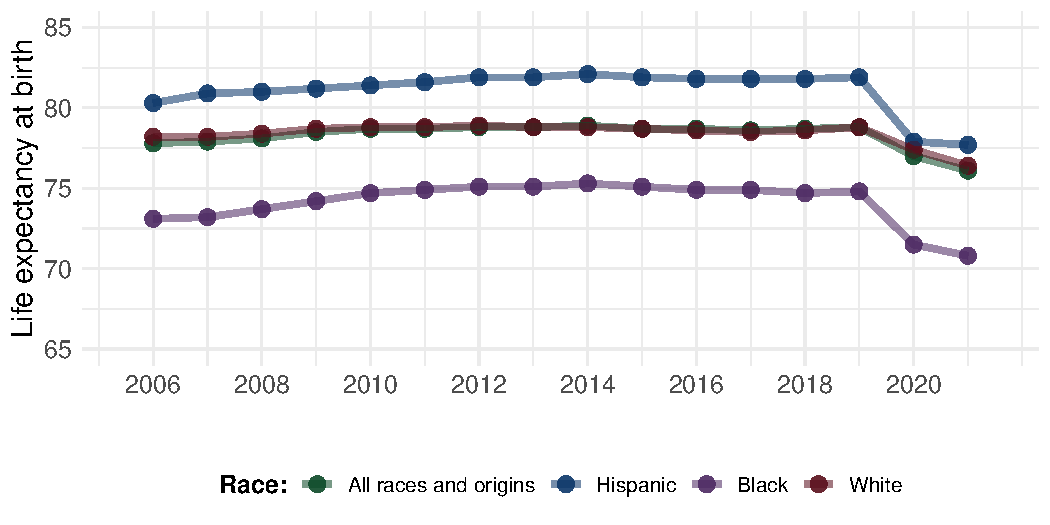
\includegraphics{paper_files/figure-pdf/fig-ELE-1.pdf}

}

\caption{\label{fig-ELE}Estimates of Life Expectancy at Birth, by Race
2006-2021}

\end{figure}

\begin{figure}

{\centering 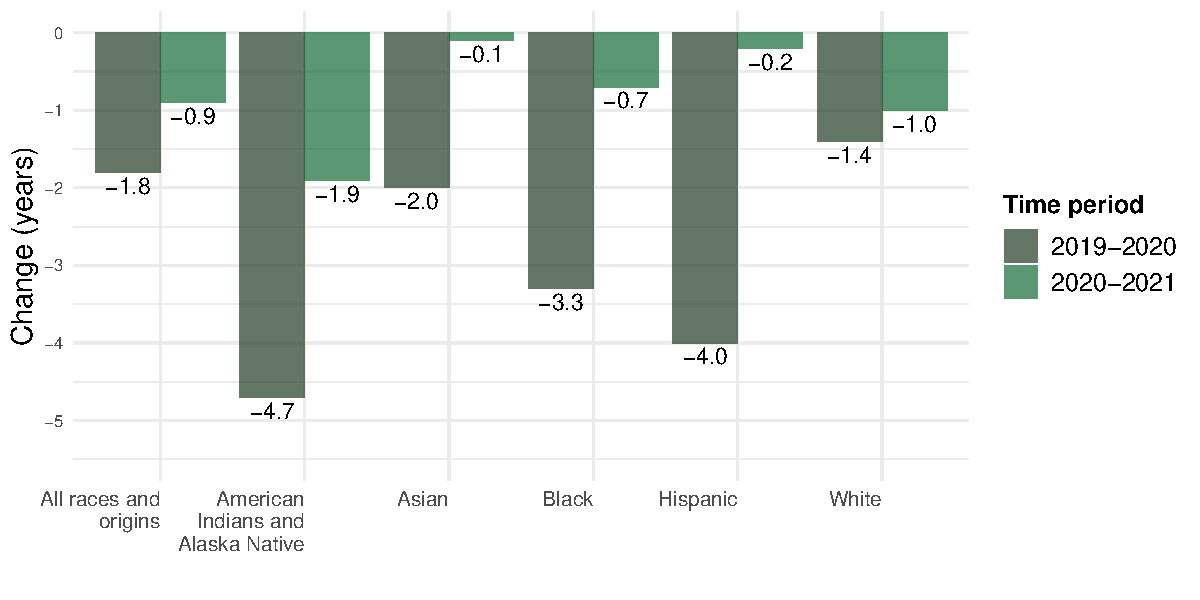
\includegraphics{paper_files/figure-pdf/fig-CLE-1.pdf}

}

\caption{\label{fig-CLE}Change in Life Expectancy at Birth from the
Previous Year}

\end{figure}

\begin{figure}

{\centering 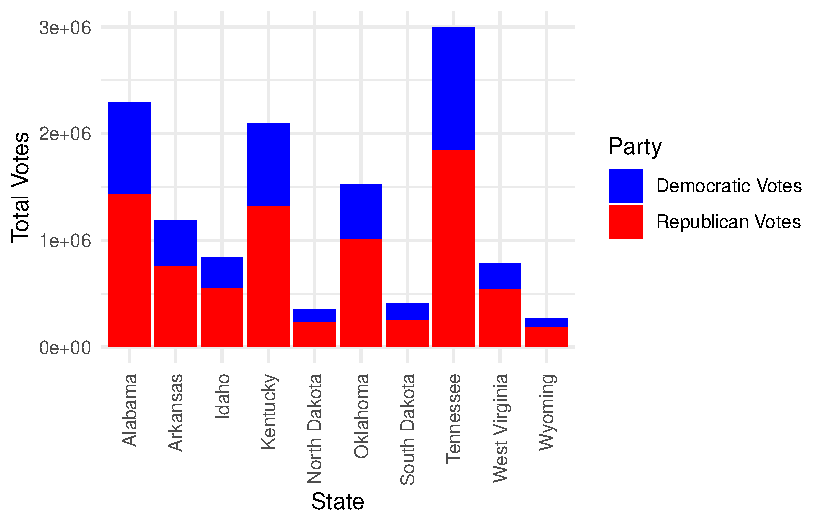
\includegraphics{paper_files/figure-pdf/fig-Vote-1.pdf}

}

\caption{\label{fig-Vote}Total Number of Votes in Top 10 States with
Highest Proportion of Republican Votes}

\end{figure}

\hypertarget{tbl-deaths}{}
\begin{longtable}{rlr}
\caption{\label{tbl-deaths}Top 10 States with Highest Death Rates from COVID-19 (per 100,000
people) }\tabularnewline

\toprule
Rank & State & Deaths \\ 
\midrule\addlinespace[2.5pt]
1 & Arizona & 455 \\ 
2 & Oklahoma & 454 \\ 
3 & Mississippi & 449 \\ 
4 & West Virginia & 444 \\ 
5 & New Mexico & 432 \\ 
6 & Arkansas & 431 \\ 
7 & Alabama & 429 \\ 
8 & Tennessee & 428 \\ 
9 & Michigan & 423 \\ 
10 & Kentucky & 406 \\ 
\bottomrule
\end{longtable}

\newpage

\hypertarget{tbl-life-exp}{}
\begin{longtable}{rrrrrrr}
\caption{\label{tbl-life-exp}Life Expectancy by Race (2019-2021) }\tabularnewline

\toprule
Year & All races and origins & Hispanic & AIAN & Asian & Black & White \\ 
\midrule\addlinespace[2.5pt]
2019 & 78.8 & 81.9 & 71.8 & 85.6 & 74.8 & 78.8 \\ 
2020 & 77.0 & 77.9 & 67.1 & 83.6 & 71.5 & 77.4 \\ 
2021 & 76.1 & 77.7 & 65.2 & 83.5 & 70.8 & 76.4 \\ 
\bottomrule
\end{longtable}

Figure~\ref{fig-CLE} serves as a valuable addition to our previous
analysis with the inclusion of Asians, American Indians, and Alaska
Natives during the critical period from 2019 to 2021. With these
additional ethnic categories, we can discern that American Indians and
Alaska Natives experienced significant impacts from the pandemic, with a
decrease of 4.7 years in the first year and 1.9 years in the second
year, totaling 6.6 years.

With a chart that depicts the change in life expectancy each year by
ethnicity, we can better gain a more comprehensive understanding of the
impact of COVID by ethnicity. While the declines in life expectancy are
smaller in magnitude from 2020 to 2021, they are notably minimal for
Asians and Hispanics, with reductions of -0.1 and -0.2 years
respectively.

Various studies have confirmed the existence of correlation between a
state's political affiliation and its handling of COVID issues (Datz
(2022)). To testify to the claim, we collected the voting data for each
of the 50 states for the 2020 presidential election. We then selected
the ten states with the highest proportions of Republican votes. These
voting patterns are visualized in Figure Figure~\ref{fig-Vote}, where
red symbols represent Republican votes and blue symbols represent
Democratic votes. Among the top ten states, Tennessee recorded the
highest total number of votes, while Wyoming boasted the highest
proportion of Republican votes.

Given the variation in population sizes among states, direct comparisons
of COVID-19 case numbers are inherently flawed. As an alternative, we
employed death rates per 100,000 people as a metric for evaluating each
state's COVID preparedness and situation. We then produced
Table~\ref{tbl-deaths} that rank the top ten states with the highest
death rates from COVID-19 per 100,000 people to examine the potential
correlation between party preferences and COVID-related deaths. Notably,
We found that six of the ten top Republican states made a reappearance
in the top death rates table; these states are Oklahoma, West Virginia,
Arkansas, Alabama, Tennessee, and Kentucky. The higher mortality rates
observed in Republican-leaning states may be attributed to their
preference for less stringent measures compared to Democratic-leaning
states, which tend to favor stricter measures (VanDusky-Allen and
Shvetsova (2021)).

Following our previous analysis regarding individuals' political
affiliations, we have developed Figure
Figure~\ref{fig-deaths-rates-votes}, which encompasses all 50 states of
the US along with their political leanings based on which party garnered
the majority votes. This information is juxtaposed against their
respective COVID-19 death rates.

While we cannot make any definitive assertions about stark differences,
we do observe that the Republican-leaning states are slightly more
clustered around higher death rates ranging from 350 to 450 deaths,
while the Democratic-leaning states appear to be more evenly
distributed, and notably one Democratic-leaning state has the lowest
death rate. An intriguing observation is that although many
Republican-leaning states demonstrate higher COVID death rates, it is
noteworthy that Arizona, typically considered a Democratic-leaning
state, records the highest death rate among all states.

\begin{figure}

{\centering 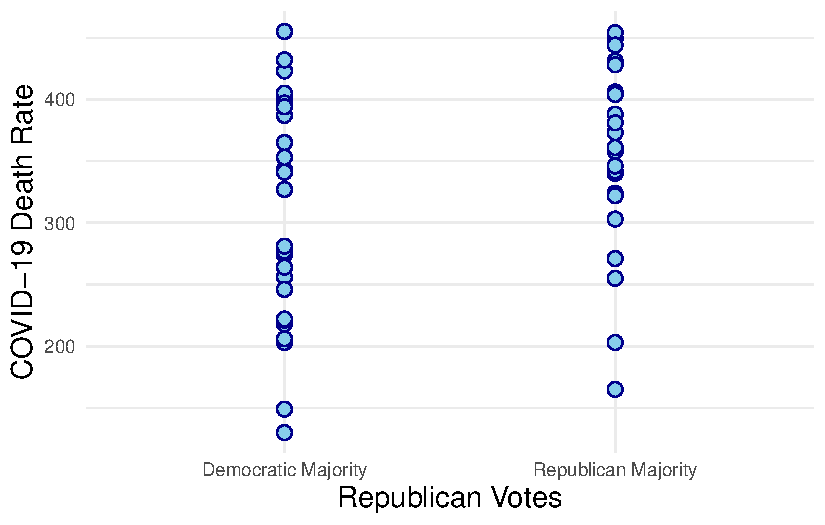
\includegraphics{paper_files/figure-pdf/fig-deaths-rates-votes-1.pdf}

}

\caption{\label{fig-deaths-rates-votes}COVID-19 Death Rates
vs.~Republican Votes}

\end{figure}

\hypertarget{discussion}{%
\section{Discussion}\label{discussion}}

This begs the question as to why we are seeing these results. There
isn't exactly a single answer to this question, however, we can
certainly point out some considerable factors to this result.

\hypertarget{influence-of-political-polarization-on-adherence-to-health-guidelines.}{%
\subsection{Influence of political polarization on adherence to health
guidelines.}\label{influence-of-political-polarization-on-adherence-to-health-guidelines.}}

Political polarization has significantly impacted the adherence to
health guidelines during the COVID-19 pandemic. The divergence in
political ideologies has translated into differing attitudes towards
health directives, including mask mandates, social distancing, and
vaccination uptake.

Various studies and our results have shown that areas with higher
support for one political party exhibited distinct behaviors and
compliance levels with health recommendations, which directly correlated
with COVID-19 case rates and mortality. A news article from
\texttt{ABC\ News} (Diab and Kumar 2023) shows that the top states with
the highest COVID-19 deaths are Arizona, and Washington with 581 deaths
and 526 deaths respectively per 100,000 people. According to 2020
presidential voting data published by \texttt{CNN}, we have both states
having the electoral vote of Democrat with Washington winning by 58\%
(\emph{2020 Election Results by State, Washington} 2020) and Arizona
winning by 49.4\% (\emph{2020 Election Results by State, Arizona} 2020).
Another news article by \texttt{ContagionLive} (Parkinson 2023) also
claims both Arizona and Washington have the highest COVID-19 mortality.
This polarization has not only influenced individual behavior but also
shaped state and local health policies, further entrenching the
disparities in health outcomes.

The adherence to health guidelines is evident in the varied health
outcomes observed across the United States. Regions with lower
compliance to health directives, often influenced by political leanings,
have experienced higher rates of COVID-19 transmission,
hospitalizations, and deaths. The disparities in vaccine uptake, driven
by political affiliations, have further exacerbated these outcomes,
leaving certain communities more vulnerable to the virus and its
variants. To mitigate the influence of political polarization on public
health, it is imperative to depoliticize health guidelines and focus on
evidence-based approaches to disease prevention and control. Building
trust in health institutions and promoting bipartisan support for public
health measures are essential steps toward achieving higher compliance
and better health outcomes. Engaging trusted community leaders and
utilizing targeted communication strategies can also help bridge the
divide and encourage adherence to health guidelines.

\hypertarget{impact-of-government-transparency-and-consistent-communication-on-public-trust.}{%
\subsection{Impact of government transparency and consistent
communication on public
trust.}\label{impact-of-government-transparency-and-consistent-communication-on-public-trust.}}

The politicization of health guidelines and mixed messages from
political and health leaders during the COVID-19 pandemic have
significantly undermined the effectiveness of public health messaging,
leading to confusion, skepticism, and eroded trust among the public.
Initially, inconsistencies in recommendations, such as on mask usage,
challenged the principle of clear, consistent, and science-based
communication essential for an effective public health response.
Moreover, the transparency of government actions and decision-making
processes is crucial in building and maintaining public trust,
especially during health crises. The level of public trust was greatly
affected by the openness and accuracy with which governments, at all
levels, communicated about the evolving situation, the reasoning behind
guidelines, and the measures taken to combat the virus, emphasizing the
importance of transparent reporting of data related to case counts,
hospitalizations, vaccine distribution, and side effects. Furthermore,
consistent communication from public health officials and government
leaders is key to ensuring adherence to health guidelines, where
inconsistencies, such as changes in mask-wearing guidelines without
clear explanations, have led to public confusion. The direct correlation
between government transparency, consistent communication, and public
behavior is self-evident, with populations receiving clear and
transparent information being more likely to adhere to guidelines,
participate in testing and tracing efforts, and accept vaccination.
Drawing lessons from the pandemic, strategies for improving government
transparency and communication in future health emergencies should
include establishing centralized information hubs, ensuring regular and
predictable communication from health authorities, engaging community
leaders in information dissemination, and harnessing digital platforms
and social media to amplify public health messages, thus reinforcing
public trust and compliance.

\hypertarget{role-of-social-vulnerabilities-and-healthcare-access-disparities-in-pandemic-impact}{%
\subsection{Role of social vulnerabilities and healthcare access
disparities in pandemic
impact}\label{role-of-social-vulnerabilities-and-healthcare-access-disparities-in-pandemic-impact}}

The COVID-19 pandemic starkly highlighted how social vulnerabilities and
disparities in healthcare access exacerbated the impact of global health
crises, contributing to significant variations in disease outcomes and
underscoring the need for targeted public health strategies that address
these disparities' root causes. Social vulnerabilities, such as
socioeconomic status, race, ethnicity, and housing conditions,
critically determined COVID-19 outcomes' severity, with populations in
crowded housing, limited access to sanitation, and lower socioeconomic
brackets experiencing higher transmission rates due to social distancing
and hygiene maintenance challenges. An independent study done by the
\texttt{Government\ of\ Canada} states that it ``identified that the
risk of COVID-19 related deaths in Black, Asian and minority ethnic
groups was nearly 1.5 times higher than White individuals'' (Emily
Thompson 2021). Another news article done by the \texttt{MSN} (Dr.
Sushama R. Chaphalkar 2024) states that `racial minority participants
reported more negative impacts on health status, activity, and absence
from work as compared to the White population.' The pandemic's economic
toll further limited these groups' healthcare access, amplifying
vulnerabilities. Disparities in healthcare access played a significant
role in influencing COVID-19 morbidity and mortality, with communities
facing healthcare facility shortages, provider scarcities, and barriers
due to insurance or financial constraints at heightened risk. These
disparities were evident in the uneven vaccine distribution and access,
highlighting the advantages of regions with strong healthcare
infrastructure. Marginalized populations, including racial and ethnic
minorities, faced compounded risks from social vulnerabilities and
healthcare disparities, evidenced by higher infection, hospitalization,
and death rates due to factors like essential service employment and
prevalent pre-existing conditions. A news article from \texttt{CNN}
(Powell 2020) talks about how many essential workers, who cannot work
from home, are from black and Latinx communities. These include
healthcare professionals, grocery cashiers, delivery workers, and public
transport employees. Despite their crucial roles, they often lack
adequate pay, protection, and respect. Addressing these disparities in
future pandemics requires public health strategies that prioritize
equity and inclusivity, including community-based healthcare
investments, enhanced vulnerable community outreach, and equitable
healthcare resource access policies. By incorporating social
determinants of health into public health preparedness plans, responses
can effectively protect at-risk populations, making future public health
responses more resilient, inclusive, and effective in safeguarding all
population segments.

\hypertarget{strategies-for-improving-real-time-data-collection-and-sharing-for-public-health-decisions.}{%
\subsection{Strategies for improving real-time data collection and
sharing for public health
decisions.}\label{strategies-for-improving-real-time-data-collection-and-sharing-for-public-health-decisions.}}

To address the fragmentation in data collection and sharing witnessed
during the pandemic, it's crucial to establish integrated data platforms
that enable seamless health data exchange among various health agencies
and stakeholders, utilizing cloud computing and APIs for real-time
accessibility and usability. Equally important is enhancing data
standardization and interoperability through universal standards like
FHIR (Fast Healthcare Interoperability Resources) to facilitate
efficient data sharing (\emph{What Is FHIR?} 2023). Investing in digital
surveillance systems, which employ AI and machine learning to sift
through diverse data sources for early outbreak detection, is essential
for rapid response to health threats. Furthermore, fostering
public-private partnerships can harness the agility of the private
sector and the public health expertise of governmental agencies to
enhance data analytics capabilities. Ensuring the privacy and security
of health data through robust governance frameworks and advanced
encryption is paramount to maintaining public trust. Engaging
communities in these initiatives ensures their relevance and fosters
trust while building global data-sharing networks encourages
international collaboration, crucial for a concerted response to
pandemics. Collectively, these strategies are fundamental to bolstering
public health decision-making and preparedness, making our health
systems more resilient against the challenges posed by emerging
infectious diseases.

\hypertarget{weaknesses-and-next-steps}{%
\subsection{Weaknesses and next steps}\label{weaknesses-and-next-steps}}

In our research, we identified several weaknesses that underscored the
gap between the U.S.'s high pandemic preparedness ranking and its actual
response to the COVID-19 crisis. Notably, there was a significant
underutilization of preparedness capacities, as the resources and
infrastructures in place were not fully mobilized or applied effectively
during the pandemic. This disconnect highlights a critical area for
improvement in aligning preparedness with real-time response
capabilities. Furthermore, the response inadequately addressed intrinsic
social vulnerabilities, exacerbating disparities in healthcare access
and outcomes among different racial and socioeconomic groups, and
underscoring the need for more inclusive and equitable public health
strategies. The heavy politicization of the pandemic response, coupled
with inconsistent messaging from health authorities, significantly
eroded public trust and compliance, emphasizing the importance of
depoliticizing public health measures and enhancing communication
strategies. Additionally, shortcomings in data and surveillance systems,
including delays in testing, inadequate genetic sequencing, and a lack
of comprehensive surveillance, hindered informed decision-making and
targeted interventions, pointing to a crucial need for investment in
data infrastructure and capabilities. The analysis also suggests that
the U.S. could benefit from more robust international benchmarking and
learning from the diverse responses of other countries to health
emergencies, which would involve understanding different strategies and
their effectiveness beyond mere outcome comparisons.

To address these challenges and strengthen the nation's resilience to
future health emergencies, several next steps are recommended.
Strengthening the linkages between preparedness and response is
imperative, ensuring that capacities are not only available but also
readily deployable and adaptable to the dynamics of a health crisis.
This includes fostering agile and responsive systems capable of rapid
mobilization. Addressing the social determinants of health is essential,
with strategies aimed at mitigating the impact of social vulnerabilities
through equitable healthcare access, support for marginalized
communities, and targeted protective measures for vulnerable
populations. Enhancing communication and public trust is vital,
necessitating clear, consistent, and transparent communication from
health authorities, alongside efforts to depoliticize health measures.
Improving data and surveillance systems is critical to providing
real-time insights, expanding genetic sequencing capabilities, and
establishing standardized data protocols. Lastly, actively engaging in
global health networks to exchange experiences, learn from global
successes and failures, and collaborate on best practices is crucial for
a more effective and equitable response that maximizes the full
potential of preparedness capacities.

\hypertarget{conclusion}{%
\section{Conclusion}\label{conclusion}}

Despite the United States' top ranking in the Global Health Security
Index as the most prepared nation for pandemics, its actual response to
the COVID-19 pandemic fell short of expectations, leading to
disproportionately high death rates. This discrepancy is attributed to
several critical factors highlighted in the paper. The U.S. did not
fully capitalize on its pandemic preparedness resources, with early
testing blunders and a lack of a unified national testing approach
hindering its response. Additionally, inherent vulnerabilities such as
the significant portion of the population in congregated settings like
nursing homes and prisons increased susceptibility to virus spread and
severe health outcomes. The politicization of the pandemic response
further compounded these issues, resulting in varied adherence to public
health guidelines across states and political lines, thereby undermining
the response's effectiveness. Moreover, inconsistent public health
communications and the challenge of accessing standardized, quality data
impeded the implementation of localized, effective interventions. The
pandemic also highlighted and intensified existing socio-economic
disparities, disproportionately impacting marginalized communities who
faced higher risks and adverse outcomes, a situation that the response
efforts failed to sufficiently mitigate.

\newpage

\hypertarget{references}{%
\section*{References}\label{references}}
\addcontentsline{toc}{section}{References}

\hypertarget{refs}{}
\begin{CSLReferences}{1}{0}
\leavevmode\vadjust pre{\hypertarget{ref-citesource3}{}}%
\emph{2020 Election Results by State, Arizona}. 2020. CNN.
\url{https://www.cnn.com/election/2020/results/state/arizona}.

\leavevmode\vadjust pre{\hypertarget{ref-citesource2}{}}%
\emph{2020 Election Results by State, Washington}. 2020. CNN.
\url{https://www.cnn.com/election/2020/results/state/washington}.

\leavevmode\vadjust pre{\hypertarget{ref-andrasfay_goldman_2022}{}}%
Andrasfay, Theresa, and Noreen Goldman. 2022. {``Reductions in US Life
Expectancy from COVID-19 by Race and Ethnicity: Is 2021 a Repetition of
2020?''} \emph{medRxiv: The Preprint Server for Health Sciences},
January, 2021.10.17.21265117.
https://doi.org/\url{https://doi.org/10.1101/2021.10.17.21265117}.

\leavevmode\vadjust pre{\hypertarget{ref-data1}{}}%
Arias, Elizabeth, Betzaida Tejada-Vera, Kenneth Kochanek, and Farida
Ahmad. 2022. {``Provisional Life Expectancy Estimates for 2021.''}
\emph{Atlanta, Georgia}, August.

\leavevmode\vadjust pre{\hypertarget{ref-data2}{}}%
Arias, Elizabeth, and Jiaquan Xu. 2022. {``United States Life Tables,
2020.''} \emph{Atlanta, Georgia}, August.

\leavevmode\vadjust pre{\hypertarget{ref-citeDataTable}{}}%
Barrett, Tyson, Matt Dowle, Arun Srinivasan, Jan Gorecki, Michael
Chirico, and Toby Hocking. 2024. \emph{Data.table: Extension of
`Data.frame`}. \url{https://CRAN.R-project.org/package=data.table}.

\leavevmode\vadjust pre{\hypertarget{ref-data3}{}}%
Bell, Julie A, and Jennifer B Nuzzo. 2021. {``Global Health Security
Index: Advancing Collective Action and Accountability Amid Global
Crisis.''} Washington D.C.:
\url{https://www.ghsindex.org/report-model/}.

\leavevmode\vadjust pre{\hypertarget{ref-citewebshot}{}}%
Chang, Winston. 2023a. \emph{Webshot: Take Screenshots of Web Pages}.
\url{https://CRAN.R-project.org/package=webshot}.

\leavevmode\vadjust pre{\hypertarget{ref-citewebshot2}{}}%
---------. 2023b. \emph{Webshot2: Take Screenshots of Web Pages}.
\url{https://CRAN.R-project.org/package=webshot2}.

\leavevmode\vadjust pre{\hypertarget{ref-data6}{}}%
\emph{COVID-19 Excess Mortality Estimates 2020-2021}. 2022. Seattle,
United States of America: Institute for Health Metrics; Evaluation
(IHME).

\leavevmode\vadjust pre{\hypertarget{ref-datz_2022}{}}%
Datz, Todd. 2022. {``Political Ideology of u.s. Elected Officials Linked
with COVID-19 Health Outcomes.''} \emph{News}.
\url{https://www.hsph.harvard.edu/news/press-releases/political-ideology-of-u-s-elected-officials-linked-with-covid-19-health-outcomes/}.

\leavevmode\vadjust pre{\hypertarget{ref-data9}{}}%
{``Death Rate, Crude (Per 1,000 People) (SP.DYN.CDRT.IN).''} 2022. The
World Bank;
\url{https://databank.worldbank.org/reports.aspx?source=2\&series=SP.DYN.CDRT.IN\&country=\#}.
2022.

\leavevmode\vadjust pre{\hypertarget{ref-citesource1}{}}%
Diab, Dr. Alaa, and Dr. Keerthana Kumar. 2023. \emph{COVID-19 Death
Rates Varied Dramatically Across US, Major Analysis Finds}. ABC News.
\url{https://abcnews.go.com/Health/covid-19-death-rates-varied-dramatically-us-major/story?id=98055024}.

\leavevmode\vadjust pre{\hypertarget{ref-data5}{}}%
Dong, Ensheng, Hongru Du, and Lauren Gardner. 2020. {``An Interactive
Web-Based Dashboard to Track COVID-19 in Real Time.''} \emph{The Lancet
Infectious Diseases} 20 (5): 533--34.
\url{https://doi.org/10.1016/S1473-3099(20)30120-1}.

\leavevmode\vadjust pre{\hypertarget{ref-citesource6}{}}%
Dr. Sushama R. Chaphalkar, PhD. 2024. \emph{COVID-19 Recovery
Disparities Uncovered Among Racial and Ethnic Groups}. MSN.
\url{https://www.msn.com/en-gb/health/other/covid-19-recovery-disparities-uncovered-among-racial-and-ethnic-groups/ar-BB1hLTLw}.

\leavevmode\vadjust pre{\hypertarget{ref-data10}{}}%
Economic, United Nations Department of, and Social Affairs Population
Division. 2022. {``World Population Prospects 2022 Demographic
Indicators by Region, Subregion and Country, Annually for 1950-2100.''}
\url{https://population.un.org/wpp/Download/Standard/MostUsed/}.

\leavevmode\vadjust pre{\hypertarget{ref-citedata2}{}}%
Elflein, John. 2023. {``U.s. COVID-19 Death Rate by State.''}
\emph{Statista}.
\url{https://www.statista.com/statistics/1109011/coronavirus-covid19-death-rates-us-by-state/}.

\leavevmode\vadjust pre{\hypertarget{ref-citesource5}{}}%
Emily Thompson, Nicole Atchessi, Rojiemiahd Edjoc. 2021. \emph{COVID-19
Race Data Collection in Canada}. The Public Health Agency of Canada.
\url{https://www.canada.ca/en/public-health/services/reports-publications/canada-communicable-disease-report-ccdr/monthly-issue/2021-47/issue-7-8-july-august-2021/covid-19-race-data-collection-canada.html}.

\leavevmode\vadjust pre{\hypertarget{ref-citeJanitor}{}}%
Firke, Sam. 2023. \emph{Janitor: Simple Tools for Examining and Cleaning
Dirty Data}. \url{https://CRAN.R-project.org/package=janitor}.

\leavevmode\vadjust pre{\hypertarget{ref-citeLubridate}{}}%
Grolemund, Garrett, and Hadley Wickham. 2011. {``Dates and Times Made
Easy with {lubridate}.''} \emph{Journal of Statistical Software} 40 (3):
1--25. \url{https://www.jstatsoft.org/v40/i03/}.

\leavevmode\vadjust pre{\hypertarget{ref-data8}{}}%
Health Statistics, National Center for. 2022. {``Life Expectancy.''} US
Centers for Disease Control; Prevention;
\url{https://www.cdc.gov/nchs/nvss/life-expectancy.htm}.

\leavevmode\vadjust pre{\hypertarget{ref-citegt}{}}%
Iannone, Richard, Joe Cheng, Barret Schloerke, Ellis Hughes, Alexandra
Lauer, and JooYoung Seo. 2024. \emph{Gt: Easily Create
Presentation-Ready Display Tables}.
\url{https://CRAN.R-project.org/package=gt}.

\leavevmode\vadjust pre{\hypertarget{ref-citedata1}{}}%
Jack, Rebecca, and Emily Oster. 2023. {``COVID-19, School Closures, and
Outcomes.''} \emph{Journal of Economic Perspectives} 37 (4): 51--70.
https://doi.org/\url{https://doi.org/10.1257/jep.37.4.51}.

\leavevmode\vadjust pre{\hypertarget{ref-citeggpubr}{}}%
Kassambara, Alboukadel. 2023. \emph{Ggpubr: 'Ggplot2' Based Publication
Ready Plots}. \url{https://CRAN.R-project.org/package=ggpubr}.

\leavevmode\vadjust pre{\hypertarget{ref-data7}{}}%
Ledesma, J R, C R Isaac, S F Dowell, D L Blazes, G V Essix, K Budeski,
Julie Bell, and Jennifer B Nuzzo. 2023. {``Evaluation of the Global
Health Security Index as a Predictor of COVID-19 Excess Mortality
Standardised for Under-Reporting and Age Structure.''} \emph{BMJ Global
Health} 8 (7): e012203. \url{https://doi.org/10.1136/bmjgh-2023-012203}.

\leavevmode\vadjust pre{\hypertarget{ref-data12}{}}%
McGovern, Tony. 2009-\/-2020. {``United States General Election
Presidential Results by County from 2009 to 2020.''} Github Repository.
\url{https://github.com/tonmcg/US_County_Level_Election_Results_08-20}.

\leavevmode\vadjust pre{\hypertarget{ref-citeHere}{}}%
Müller, Kirill. 2020. \emph{Here: A Simpler Way to Find Your Files}.
\url{https://CRAN.R-project.org/package=here}.

\leavevmode\vadjust pre{\hypertarget{ref-citeRColorBrewer}{}}%
Neuwirth, Erich. 2022. \emph{RColorBrewer: ColorBrewer Palettes}.
\url{https://CRAN.R-project.org/package=RColorBrewer}.

\leavevmode\vadjust pre{\hypertarget{ref-citearticle}{}}%
Nuzzo, Jennifer B., and Jorge R. Ledesma. 2023. \emph{Why Did the Best
Prepared Country in the World Fare so Poorly During COVID?}
\url{https://www.aeaweb.org/articles?id=10.1257/jep.37.4.3}.

\leavevmode\vadjust pre{\hypertarget{ref-citesource4}{}}%
Parkinson, John. 2023. \emph{Which States Saw Greatest COVID-19
Mortality?} ContagionLive.
\url{https://www.contagionlive.com/view/which-states-saw-greatest-covid-19-mortality-}.

\leavevmode\vadjust pre{\hypertarget{ref-citeSF}{}}%
Pebesma, Edzer. 2018. {``{Simple Features for R: Standardized Support
for Spatial Vector Data}.''} \emph{{The R Journal}} 10 (1): 439--46.
\url{https://doi.org/10.32614/RJ-2018-009}.

\leavevmode\vadjust pre{\hypertarget{ref-citesource7}{}}%
Powell, Catherine. 2020. \emph{Color of Covid: The Racial Justice
Paradox of Our New Stay-at-Home Economy}. CNN.
\url{https://www.cnn.com/2020/04/10/opinions/covid-19-people-of-color-labor-market-disparities-powell/index.html}.

\leavevmode\vadjust pre{\hypertarget{ref-citeR}{}}%
R Core Team. 2022. \emph{R: A Language and Environment for Statistical
Computing}. Vienna, Austria: R Foundation for Statistical Computing.
\url{https://www.R-project.org/}.

\leavevmode\vadjust pre{\hypertarget{ref-data4}{}}%
Systems Science, Center for, and Engineering. 2023. {``COVID-19
Dashboard.''} John Hopkins University.

\leavevmode\vadjust pre{\hypertarget{ref-vandusky-allen_shvetsova_2021}{}}%
VanDusky-Allen, Julie, and Olga Shvetsova. 2021. {``How America's
Partisan Divide over Pandemic Responses Played Out in the States.''}
\emph{The Conversation}.
\url{https://theconversation.com/how-americas-partisan-divide-over-pandemic-responses-played-out-in-the-states-157565}.

\leavevmode\vadjust pre{\hypertarget{ref-data11}{}}%
Wang, Haidong, Kara R Paulson, Samuel A Pease, Samuel Watson, Haley
Comfort, Pu Zheng, A Y Aravkin, et al. 2022. {``Estimating Excess
Mortality Due to the COVID-19 Pandemic: A Systematic Analysis of
COVID-19-Related Mortality, 2020--21.''} \emph{The Lancet} 399 (10334):
1513--36. \url{https://doi.org/10.1016/S0140-6736(21)02796-3}.

\leavevmode\vadjust pre{\hypertarget{ref-citesource8}{}}%
\emph{What Is FHIR?} 2023. The Office of National Coordinator for Health
Information Technology.
\url{https://www.healthit.gov/sites/default/files/2019-08/ONCFHIRFSWhatIsFHIR.pdf}.

\leavevmode\vadjust pre{\hypertarget{ref-citeggplot}{}}%
Wickham, Hadley. 2016. \emph{Ggplot2: Elegant Graphics for Data
Analysis}. Springer-Verlag New York.
\url{https://ggplot2.tidyverse.org}.

\leavevmode\vadjust pre{\hypertarget{ref-citeTidyVerse}{}}%
Wickham, Hadley, Mara Averick, Jennifer Bryan, Winston Chang, Lucy
D'Agostino McGowan, Romain François, Garrett Grolemund, et al. 2019.
{``Welcome to the {tidyverse}.''} \emph{Journal of Open Source Software}
4 (43): 1686. \url{https://doi.org/10.21105/joss.01686}.

\leavevmode\vadjust pre{\hypertarget{ref-citeReadXL}{}}%
Wickham, Hadley, and Jennifer Bryan. 2023. \emph{Readxl: Read Excel
Files}. \url{https://CRAN.R-project.org/package=readxl}.

\leavevmode\vadjust pre{\hypertarget{ref-citeDplyr}{}}%
Wickham, Hadley, Romain François, Lionel Henry, Kirill Müller, and Davis
Vaughan. 2023. \emph{Dplyr: A Grammar of Data Manipulation}.
\url{https://CRAN.R-project.org/package=dplyr}.

\leavevmode\vadjust pre{\hypertarget{ref-citeScales}{}}%
Wickham, Hadley, Thomas Lin Pedersen, and Dana Seidel. 2023.
\emph{Scales: Scale Functions for Visualization}.
\url{https://CRAN.R-project.org/package=scales}.

\leavevmode\vadjust pre{\hypertarget{ref-citeKnitR}{}}%
Xie, Yihui. 2014. {``Knitr: A Comprehensive Tool for Reproducible
Research in {R}.''} In \emph{Implementing Reproducible Computational
Research}, edited by Victoria Stodden, Friedrich Leisch, and Roger D.
Peng. Chapman; Hall/CRC.

\leavevmode\vadjust pre{\hypertarget{ref-citeKableExtra}{}}%
Zhu, Hao. 2024. \emph{kableExtra: Construct Complex Table with 'Kable'
and Pipe Syntax}. \url{https://CRAN.R-project.org/package=kableExtra}.

\end{CSLReferences}



\end{document}
